\chapter{Adding dense point data (own data with geometry)}

\pagestyle{fancy}
\fancyhf{}
\fancyhead[OC]{\leftmark}
\fancyhead[EC]{\rightmark}
%\renewcommand{\footrulewidth}{1pt}
\cfoot{\thepage}

%%%%%%%%%%%%%%%%%%%%%%%%%%%%%%%%%%%%%%%%%%%%%%%%%%%%%%%%%%%
%%%%%%%%%%%%%%%%%%%%%%%%%%%%%%%%%%%%%%%%%%%%%%%%%%%%%%%%%%%

\section{Data}

\textit{We've yet to present data of this type, but it seems this is a very popular datatype for police, so here's an introduction. Please use the vast amount of online tutorials to find out more.}\\

Filename to use for this section: $sw\_5forces\_stop\_and\_search.csv$

\begin{figure}[!h]
	\centering
	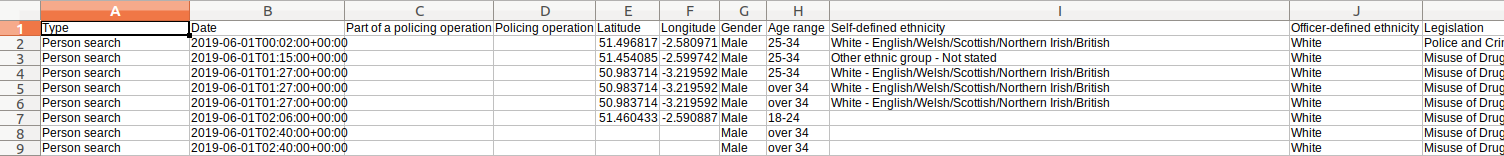
\includegraphics[width=1\textwidth]{images/image1.png}
	\caption{CSV file containing 38,832 stop and search instances over 3 years}
	\label{ft_fig_firstfig3}
\end{figure}

File contains our own geographical data regarding 38,832 stop and search instances over 3 years.\\
15 fields including: latitude, longitude and gender.\\
QGIS can simply take lat and long and plot point on map.\\
Tip: If get Lat and Long the wrong way round then your points will be in Africa!

\section{Add delimited text layer}

Opening a csv file is known as \textit{adding a delimited text layer}. There are many ways to do this:
\begin{enumerate}[~~~1)]
	\item
	Menu: Layer $\rightarrow$ Add Layer $\rightarrow$ Add Delimited Text Layer	
	\item 
	\textit{Add delimited text layer} icon on a toolbar
	\begin{tabular}{@{}c@{}}
\includegraphics[width=4ex]{images/add_delimited_text_layer_icon.png}\end{tabular}
	\item 
	Use \textit{browse panel} to navigate to the file location
	\item 
	Data Source Manager icon
	\begin{tabular}{@{}c@{}}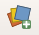
\includegraphics[width=4ex]{images/data_source_manager_icon.png}\end{tabular}
\end{enumerate}

Within the \textit{Data Source Manager / Delimited text} window, choose these settings:\\
\textbf{File name:} Navigate to the csv file: $sw\_5forces\_stop\_and\_search.csv$\\
\textbf{Layer name} (what appears in the \textit{Layers Panel}, so choose something meaningful): stop\_search\\
\textbf{File Format}: CSV (comma separated values)\\
\textbf{Geometry definition} $\rightarrow$ Point coordinates $\rightarrow$  
\textbf{x field} = Longitude \& \textbf{y field} = Latitude\\
\textbf{Coordinate system}: EPSG4326 – WGS 84 (leave as default)\\
(Note: The top row of the csv file is used as the field titles.)\\
\textbf{Add}.\\

\begin{figure}[!h]
	\centering
	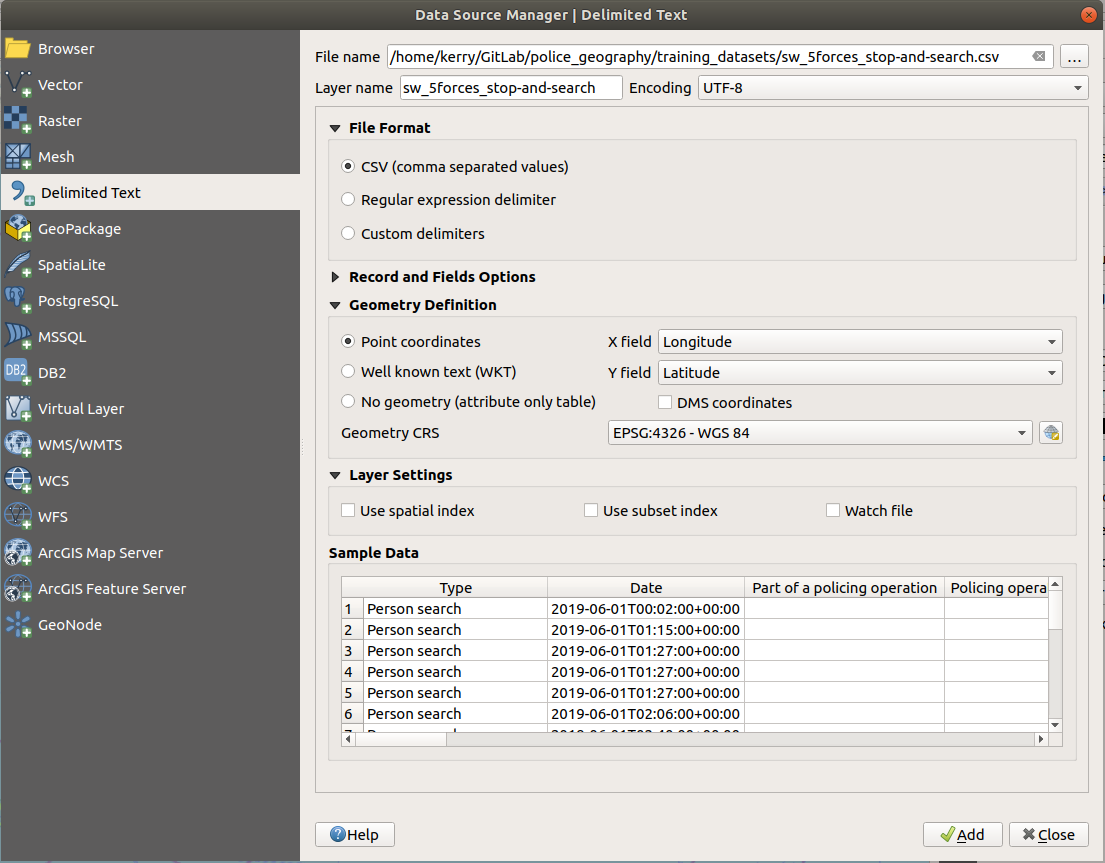
\includegraphics[width=0.6\textwidth]{images/add_delimited_text_stop_and_search.png}
	\caption{\textit{Data Source Manager / Delimited text} window}
	\label{ft_fig_firstfig3}
\end{figure}
%\null\newpage

All of the 38,832 instances will will be added to your map canvas as points.\\

\begin{figure}[!h]
	\centering
	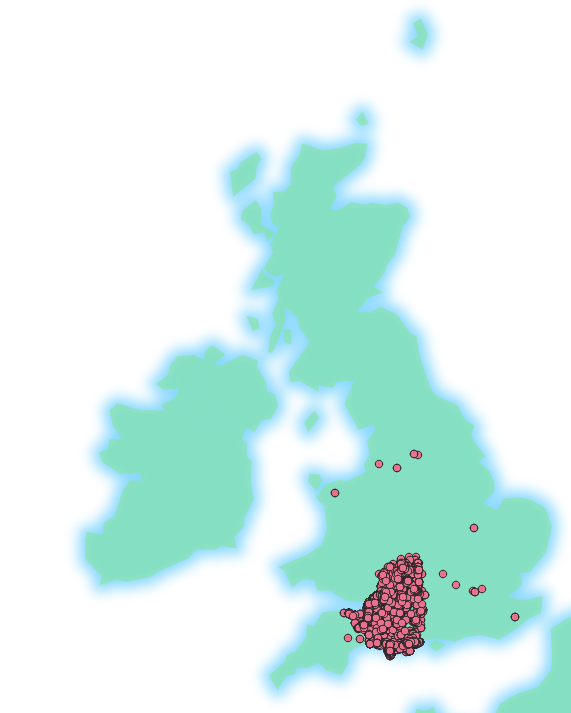
\includegraphics[width=0.4\textwidth]{images/stop_search_38832_points_over_uk.png}
	\caption{Stop and search points added to our base map}
	\label{ft_fig_firstfig3}
\end{figure}

Instantly see a benefit for plotting geographical data in a mapping software: highlights oddities. This is the dataset for the 5 SW forces. I'm curious, is there a reason why the points exist outside this region?\\

The layer name will exist in the \textit{Layers Panel}. Make sure the stop\_search layer name is above the UK base map layer.\\
Play with changing the order of the layers within the \textit{Layers Panel} (drag and drop).\\

\section{Attribute table}

As we saw for the World base map layer, each layer open in the project has an \textit{attribute table}. For this layer, each point on the map has a row of data in the layer's \textit{attribute table}.

\subsection{Open attribute table}

To open a layer's \textit{attribute table}, make sure the relative layer is highlighted in the \textit{Layers Panel}, and then click	\begin{tabular}{@{}c@{}}
\includegraphics[width=4ex]{images/attribute_table_icon.png}\end{tabular}
in the top toolbar.\\
Or right click on layer name in the \textit{Layers Panel} and select \textit{Open Attribute Table}.

\begin{figure}[!h]
	\centering
	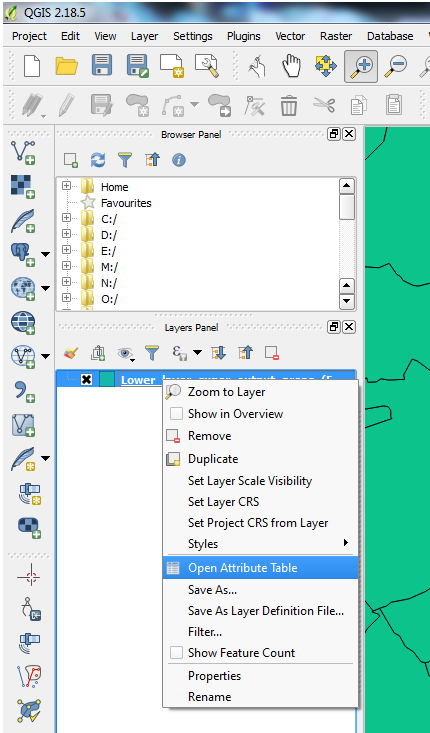
\includegraphics[width=0.3\textwidth]{images/right_click_layername.png}
	\caption{Open attribute table}
	\label{ft_fig_firstfig3}
\end{figure}

The data in the \textit{attribute table} is essentially the csv file. Can sort the data (like in excel) by clicking on the title row.\\
In GIS software, variables (columns) are referred to as \textit{fields},and rows as \textit{features}.\\

\begin{figure}[!h]
	\centering
	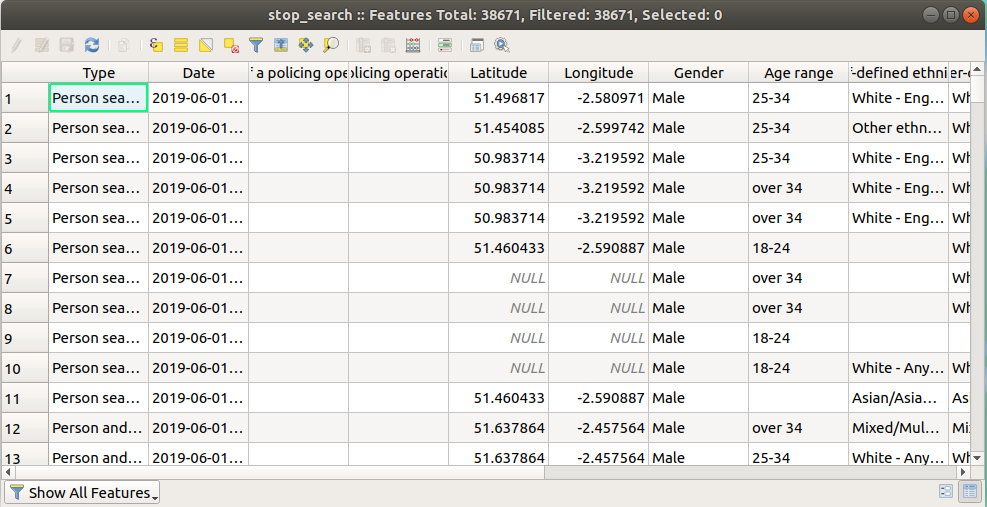
\includegraphics[width=0.6\textwidth]{images/stop_search_attribute_table.png}
	\caption{Attribute table for Stop Search layer}
	\label{ft_fig_firstfig3}
\end{figure}

\null\newpage

\subsection{Relationship between the attribute table and the map canvas}
For data with many points, it is often the case that many points will lie in the same space. So even when you have a point highlighted, it may be hidden under another point and so not visible on your map.

\subsubsection{From attribute table to map canvas}
Can select row(/s) in attribute table and see where they are in the map canvas (they become highlighted in yellow on the map - unless the point is under another point).\\

Select a row (point) in the attribute table. Notice the \textit{Attribute table} window title reports the number of total features, and any selected.\\

\begin{figure}[!h]
	\centering
	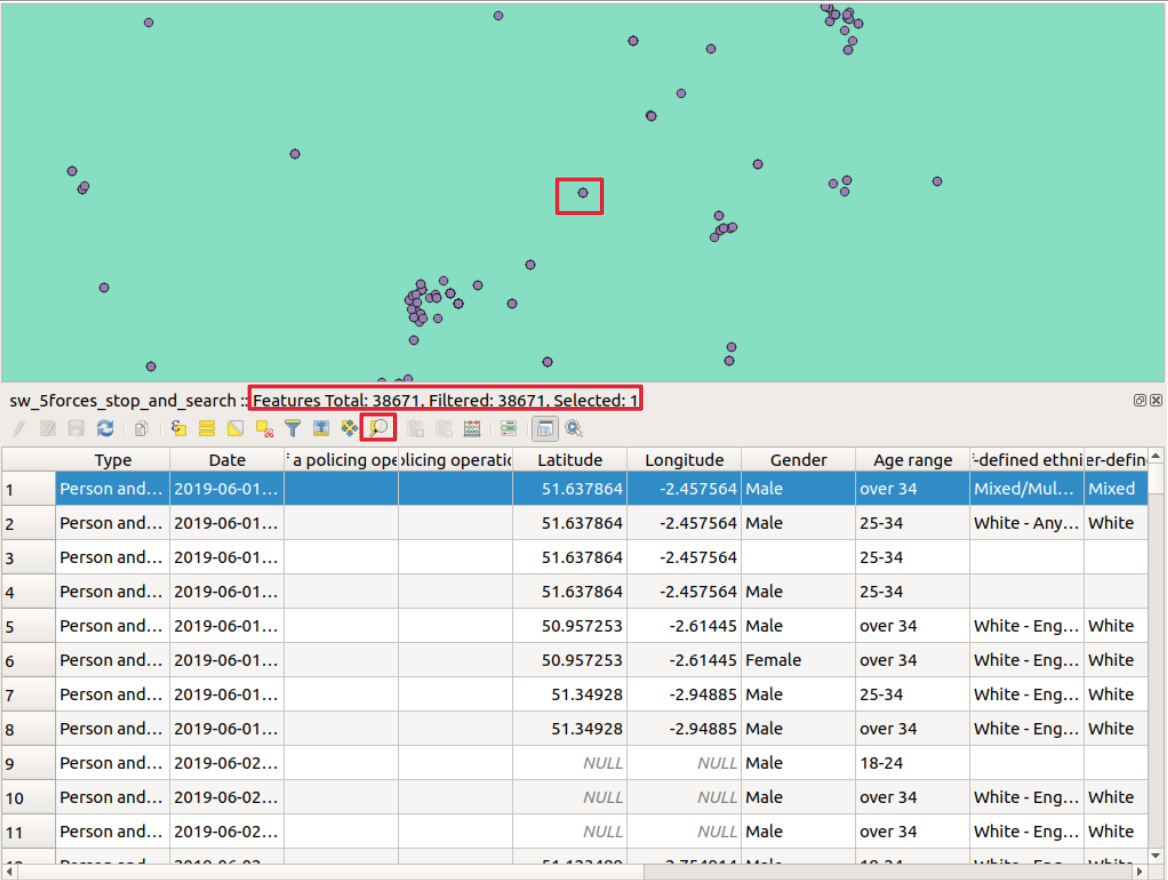
\includegraphics[width=0.5\textwidth]{images/stop_search_one_row_selected_redbox.png}%stop_search_at_tbl_select_6_features_redbx.png}%attribute_table_top_rows.png}
	\caption{Stop and search attribute table, selected 1 row with relevant point highlighted, not in yellow as it's under another point. Red boxes highlight 1) Point selected 2) Number of features selected 4) Zoom to point button}
	\label{ft_fig_firstfig3}
\end{figure}

Sometimes we can not instantly see where these features are on our map, so use the map navigation function buttons: \textit{Pan to selected} \& \textit{Zoom to selected}. These function buttons are in the Attributes \& Map Navigation toolbars, and in the Attribute Table title bar. For some cases, need to press this button a couple of times for it to take effect.

\begin{figure}[!h]
	\centering
	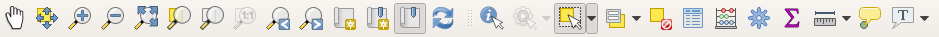
\includegraphics[width=1\textwidth]{images/attribute_and_map_navigation_toolbars_icons.png}
	\caption{Function buttons in the Attributes \& Map Navigation toolbars}
	\label{ft_fig_firstfig3}
\end{figure}

Useful to know at this stage that we can dock the attribute table to the main window, so we can see both the map canvas and the attribute table 
\begin{tabular}{@{}c@{}}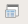
\includegraphics[width=4ex]{images/dock_attribute_table_icon.png}\end{tabular}\\

If no yellow point exists, then it will be under another point.
A useful tool to then use is Identify Feature tool. See the next section.\\
\null\newpage
To get an example which only has one point at a location (so can see the yellow selected point) sort the attribute table by the field \textit{Date}, select the top row and Zoom To Selected.
\begin{figure}[!h]
	\centering
	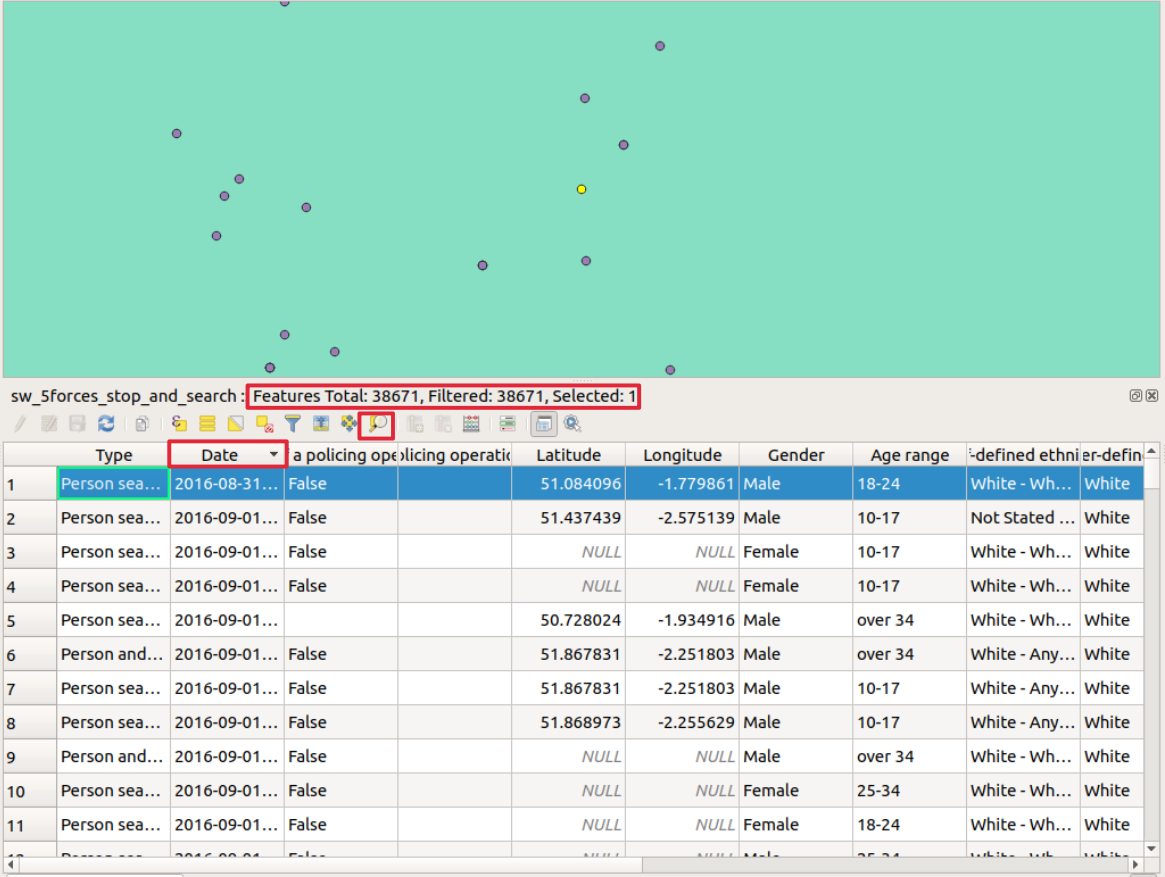
\includegraphics[width=0.5\textwidth]{images/stop_search_one_row_selected_oldest_date_redbox_docked_at_table.png}%stop_search_one_row_selected_oldest_date_redbox.png}%stop_search_at_tbl_select_6_features_redbx.png}%attribute_table_top_rows.png}
	\caption{Stop and search attribute table. Red boxes highlight 1) Order by Date 2) Selecting the oldest feature 3) Number of features selected 4) Map navigation function buttons}
	\label{ft_fig_firstfig3}
\end{figure}


\subsubsection{From map canvas to attribute table using the \textit{Identify Feature} tool}

Click the \textit{Identify Feature} icon 
\begin{tabular}{@{}c@{}}
\includegraphics[width=4ex]{images/identify_feature_icon.png}\end{tabular}

This function will only work on the top layer (as in the \textit{Layers Panel}, even if the top layer is unselected.

Click on a feature (point). Information about that feature (point) will be displayed in the \textit{Identify Results Panel}, this is essentially the values of the fields in the layer's \textit{Attribute Table}):  

\begin{figure}[!h]
	\centering
	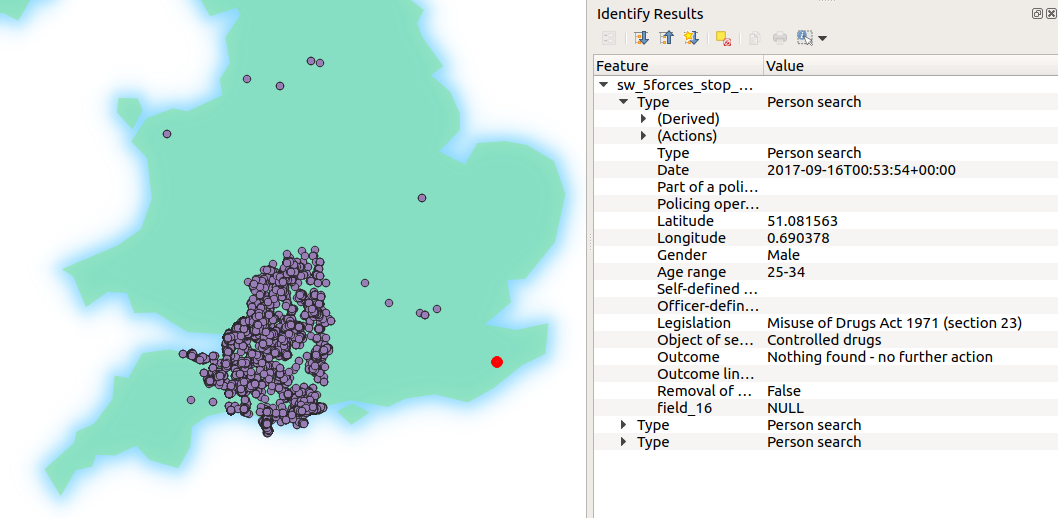
\includegraphics[width=0.55\textwidth]{images/stop_search_identify_feature.png}%identify_feature_window.png}
	\caption{Identify features tool, and panel}
	\label{ft_fig_firstfig3}
\end{figure}

For locations with multiple points on the same site, all of the features will appear in the \textit{Identify Results Panel}.

\subsubsection{From map canvas to attribute table using the \textit{Select Feature(s)} tool}

Alternatively, can select feature(s) (points) on the map using the \textit{Select Feature(s)} tool, the icon is in the top toolbar
\begin{tabular}{@{}c@{}}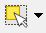
\includegraphics[width=4ex]{images/select_features_by_polygon_icon.png}\end{tabular}
, (right click to end selection).

\begin{figure}[!h]
	\centering
	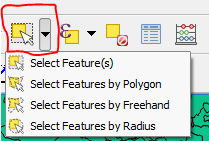
\includegraphics[width=0.2\textwidth]{images/select_features_by_polygon_dropdown.png}
	\caption{Options for the Select Feature(s) tool}
	\label{ft_fig_firstfig3}
\end{figure}

View the field values in the \textit{Attribute Table}, and move selection to top
\begin{tabular}{@{}c@{}}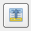
\includegraphics[width=4ex]{images/move_selection_to_top_icon.png}\end{tabular}


\begin{figure}[!h]
	\centering
	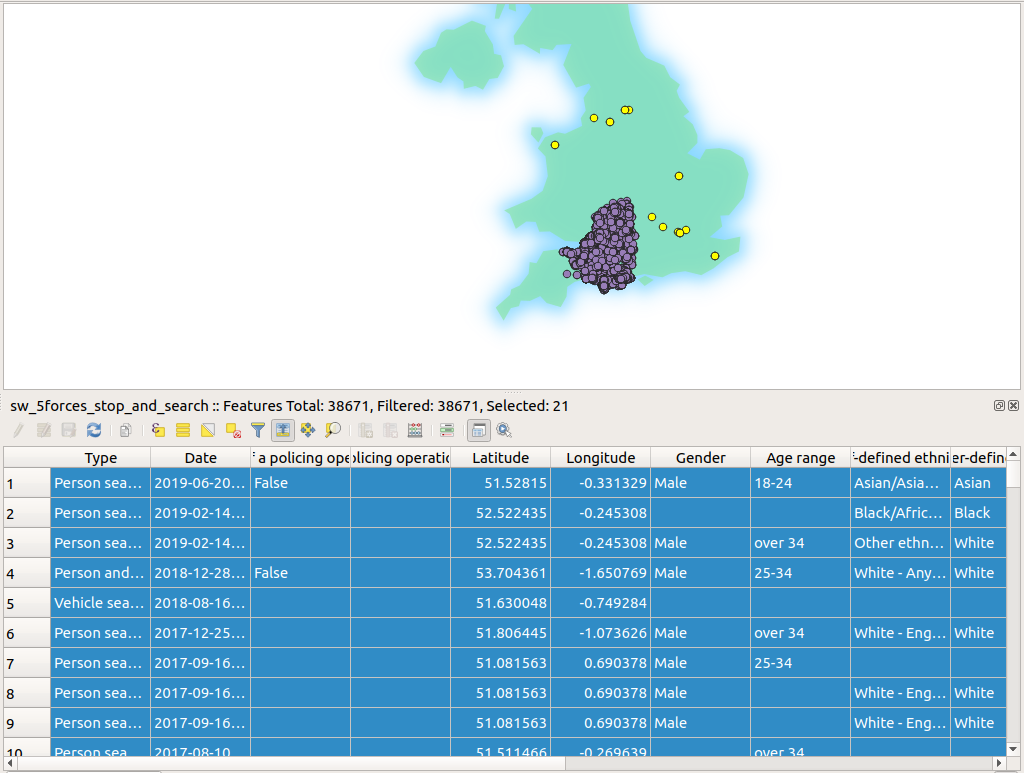
\includegraphics[width=0.5\textwidth]{images/stop_search_select_features.png}
	\caption{Selecting the outlying points, and bringing those features to the top of the attribute table}
	\label{ft_fig_firstfig3}
\end{figure}
\null\newpage

Close Attribute Table (x in top right of window)\\
Close Identify Results panel \& Deselect all features.\\
% Not needed, done in world. INTRODUCE AND USE LAYER STYLING TO CHANGE THE SIMPLE SYMBOL.

% Not needed, done in sparse pt. SYMBOLOGY CATEGORIZED.

%\section{Symbology: Categorized}
%
%We've already explored how to use the \textit{Layers Styling Panel} to change the style of a \textit{Single symbol} (to get the coastline and landmass of UK). Let's now look at how to add symbology to a layer based on a categorical field value, such as gender.\\
%
%In the \textit{Layer Styling Panel}, select from the dropdown \textit{Categorized}\\
%Column: \textit{Gender}\\
%Classify.\\
%
%If only interested in the division between Female, Male and Other, can deselect the "all other categories".
%
%Also for each category, double click on the symbol (next to the corresponding value), select "Simple marker" to alter the size and colour of the point.
%
%\begin{figure}[!h]
%	\centering
%	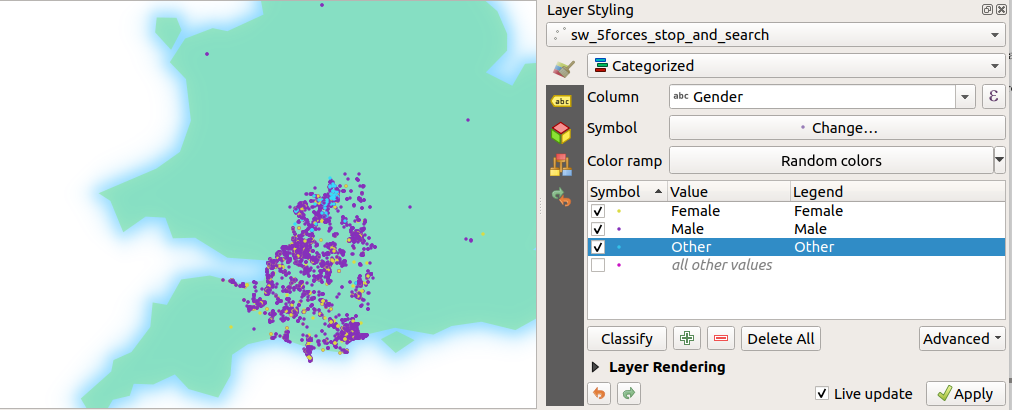
\includegraphics[width=0.7\textwidth]{images/stop_search_categorized.png}%stop_search_pt_data_gender.png}
%	\caption{}
%	\label{ft_fig_firstfig3}
%\end{figure}
%
%\begin{figure}[!h]
%	\centering
%	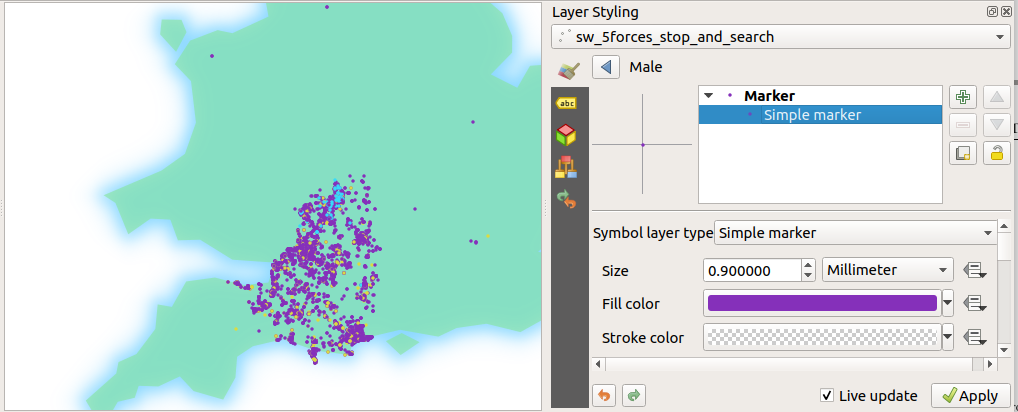
\includegraphics[width=0.7\textwidth]{images/stop_search_categorized_simple_marker.png}%stop_search_38832_points.png}
%	\caption{}
%	\label{ft_fig_firstfig3}
%\end{figure}
%

\section{Symbology for dense point data}

For dense point data (with many points at the same location) there are at least two options available.

\subsection{Heatmap}
In the \textit{Layer Styling Panel}, select in the dropdown: \textit{Heatmap}.
Play with the color ramp (I quite like \textit{magma} for heatmap), radius, units, and opacity (expand Layer rendering).

\begin{figure}[!h]
	\centering
	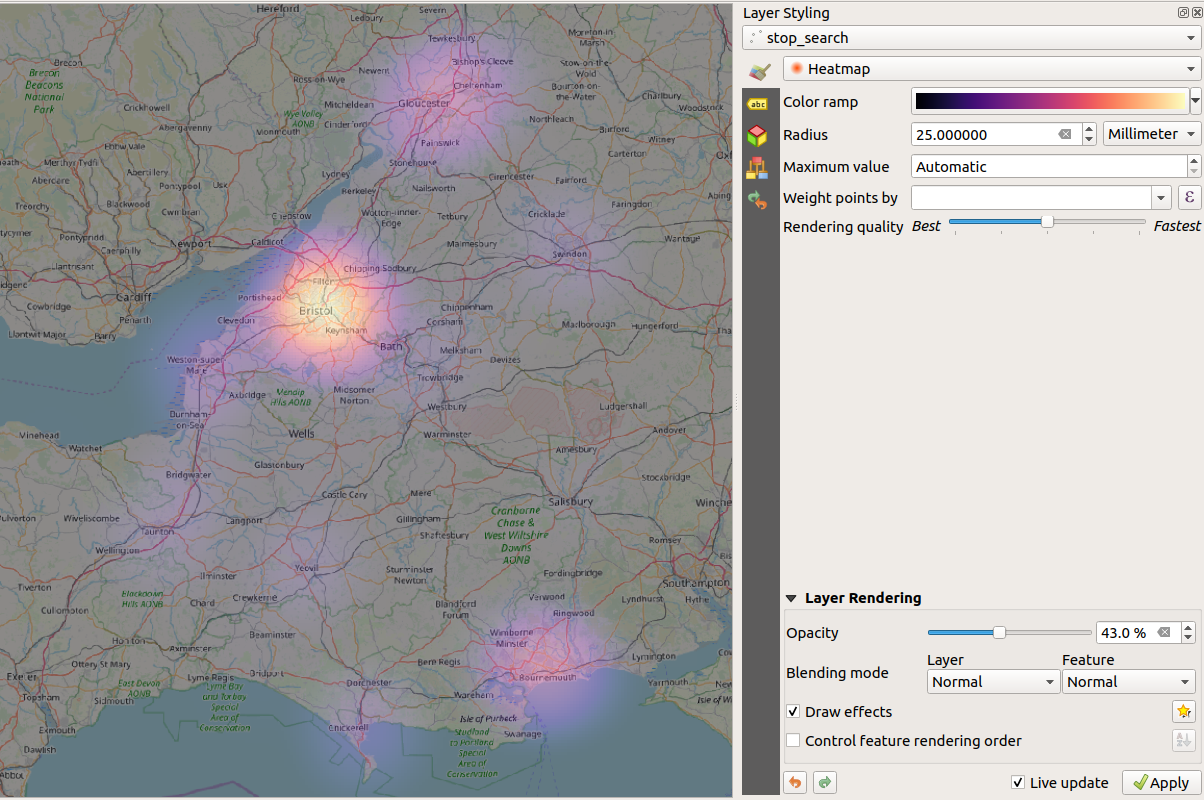
\includegraphics[width=0.5\textwidth]{images/heatmap3.png}
	\caption{Heatmap for the stop and search dataset}
	\label{ft_fig_firstfig3}
\end{figure}

For more information on styling heatmaps see \url{https://www.qgistutorials.com/en/docs/3/creating_heatmaps.html}, where the example data is conveniently about crimes.

\subsection{Point Cluster Renderer}

Create a duplicate of layer \textit{stop\_search} and rename layer.\\
This option is inspired by the maps I saw on the police website:\\ \url{https://www.police.uk/devon-and-cornwall/DEV.4055/crime/}.\\
I found this tutorial helpful: \url{https://www.youtube.com/watch?v=-ikF1oYIpa0}\\

In the \textit{Layer Styling Panel}, select in the dropdown: \textit{Point cluster}.\\

Experiment with the settings to get an uncluttered map where the points don't overlap and make it look too busy.

\begin{figure}[!h]
	\centering
	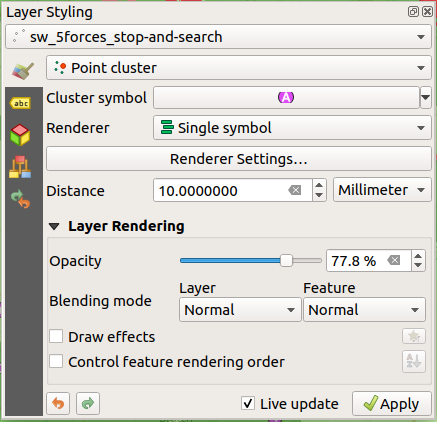
\includegraphics[width=0.3\textwidth]{images/point_cluster_layer_styling_panel.png}
	\caption{Layer Styling pane showing the settings available for Point cluster}
	\label{ft_fig_firstfig3}
\end{figure}


Distance units: \textit{Millimetre or Inches} - the points join together based on the scale. \textit{Map units, pixels or point} - the points that are joined together are fixed.\\

Can also change point size depending on number:\\
Cluster symbol $\rightarrow$ Simple marker $\rightarrow$ Size $\rightarrow$ Assistant $\rightarrow$ Source: $"@cluster\_size"$\\

Experiment with the range of "Values from" and "to". Also "Size from" and "to".\\


\begin{figure}[h!] % "[t!]" placement specifier just for this example
	\begin{subfigure}{0.48\textwidth}
		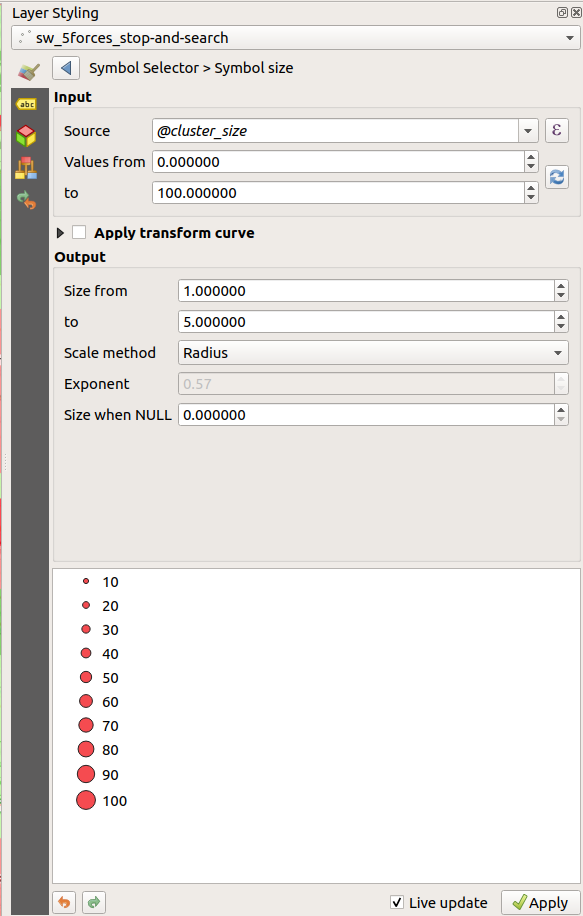
\includegraphics[width=0.6\textwidth]{images/point_clustering_cluster_size.png}
		\caption{Settings to make the point size change depending on the number of points in the cluster}
		\label{ft_fig_firstfig3}
	\end{subfigure}\hspace*{\fill}
	\begin{subfigure}{0.48\textwidth}
		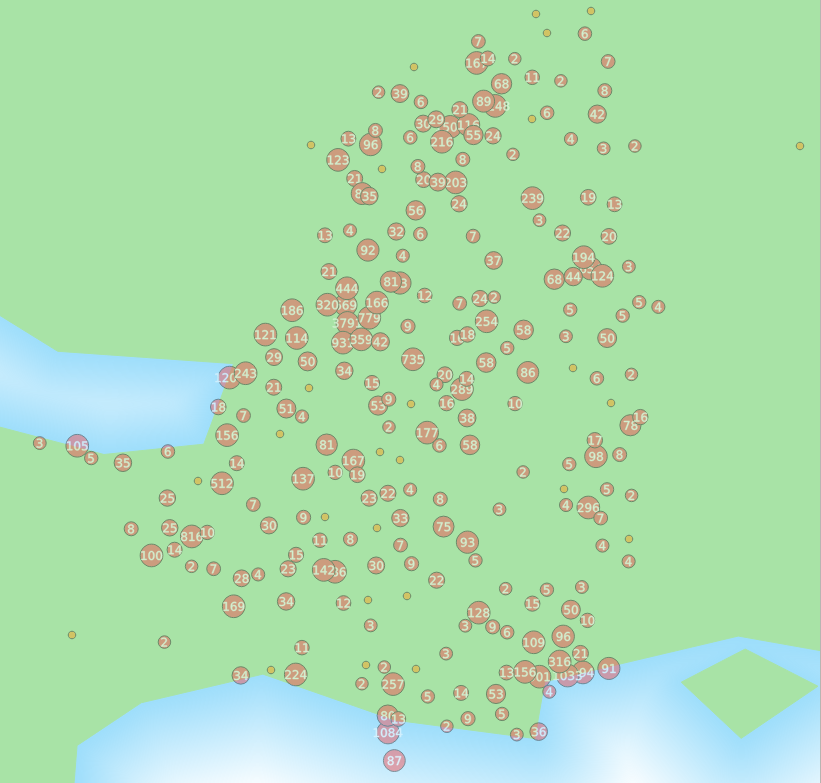
\includegraphics[width=1\textwidth]{images/point_cluster_map.png}
		\caption{Point cluster symbology}
		\label{ft_fig_firstfig3}
	\end{subfigure}
\end{figure}

%\begin{figure}[!h]
%	\centering
%	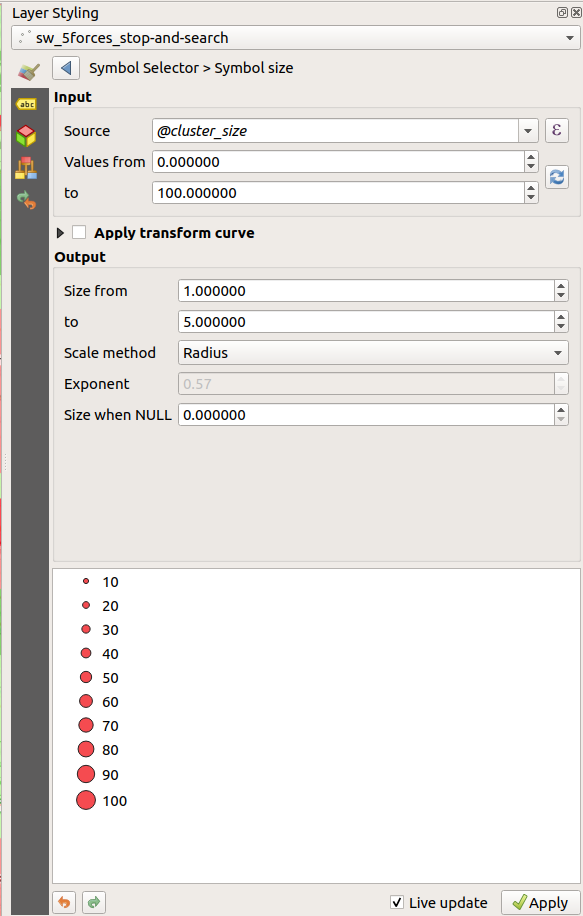
\includegraphics[width=0.3\textwidth]{images/point_clustering_cluster_size.png}
%	\caption{Settings to make the point size change depending on the number of points in the cluster}
%	\label{ft_fig_firstfig3}
%\end{figure}
%


Unselect the stop\_search layer in the \textit{Layers} panel.